    To perform our analysis of network-level, geographic, and service isolation in face of large-scale physical disaster, we generated a model of AS connectivity which incorporates physical locations of AS peering, and maps ASes to geographic regions they serve. 
    We develop our dataset by borrowing techniques and data from
    the IXP
    Mapping Project~\cite{ixps-mapped}, iPlane~\cite{iplane},
    Aqualab~\cite{sidewalk},
    CAIDA~\cite{caidadata}, and the MaxMind~\cite{maxmind} and
IP2Location~\cite{ip2loc} industrial IP geolocation services.

    To model connectivity, we generate an AS-level graph with hyperedges for
each PoP or {\it failure point} where ASes connect.
    Thus, a pair of ASes may be joined by multiple edges if they peer in
redundant physical locations.
    Further, a single hyperedge may join two or more ASes when many ASes
converge on a the same location for peering.
    \justine{figure?}
    
    We use a measurement-based technique borrowed from iPlane~\cite{iplane}
generate a graph representing real world peering arrangements.  
    Our starting dataset was a set of traceroutes issued through June and July 2010 by
iPlane~\cite{iplane} and Aqualab~\cite{aqualab}, and CAIDA's~\cite{caida} July
2010 Internet Topology Datakit.
    We then mapped IP addresses which appeared adjacent to eachother in the
router-level topology to their AS numbers. 
    We collected all IP addresses which we identified as `border routers', that
is, that connected to an IP address which we identified as belonging to another
AS.
    We issued UDP pings to each of the border routers from 134
PlanetLab~\cite{planetlab} nodes and used the TTL values from the replies to
generate estimated reverse path lengths for each node. 
    We also geolocated each IP address using a combination of the
MaxMind~\cite{maxmind} and IP2Location~\cite{ip2loc} industrial geolocation
services.
    Using these TTL values and geolocated latitudes and longitudes, we used
a modified version of iPlane's~\cite{iplane} PoP-detection algorithm.
    The technique generates clusters based on both geolocation and similar
TTL-values. 
    However, where iPlane creates PoPs which only contain IP addresses from a
single AS, we allowed multiple ASes to be clustered into the same PoP. 
    For each resulting PoP, we created a hyperedge including all of the ASes
with IP addresses within the PoP, and annotated it with the assigned geographic
location.

    The resulting graph contained {\bf n} PoPs with an average of {\bf m}
ASes... \justine{describe dataset}. 

    We then annotated each AS with a geographic `coverage' region, to provide
an estimate of the area served by each network. 
    To do this, we sampled \justine{a fraction} of each network's IP space and
once again geolocated each address. 
    We then used our sampling to generate a (latitude, longitude) bounding box
around the region served.    
    \justine{describe dataset}.
    \justine{refer to figure}.
    \justine{For class project: let's calculate some Chernoff bounds so that we
can be smart about our sample, given that MaxMind estimates 83\% accuracy?}
 
        \subsubsection*{Evaluation of Model}
            \begin{itemize}
        \item survey random network providers and ask them if what we
        found was correct
        \item Compare iPLaney data to Brice (Manual) Data.
        \item compare physical links discovered to logical connectivity
        graph (CAIDA provides this) - what fraction of logical links
        did we observe? For Tier-1's? For Tier-2's? For stub networks?
            \end{itemize} 

\begin{figure}[tb]
\centering
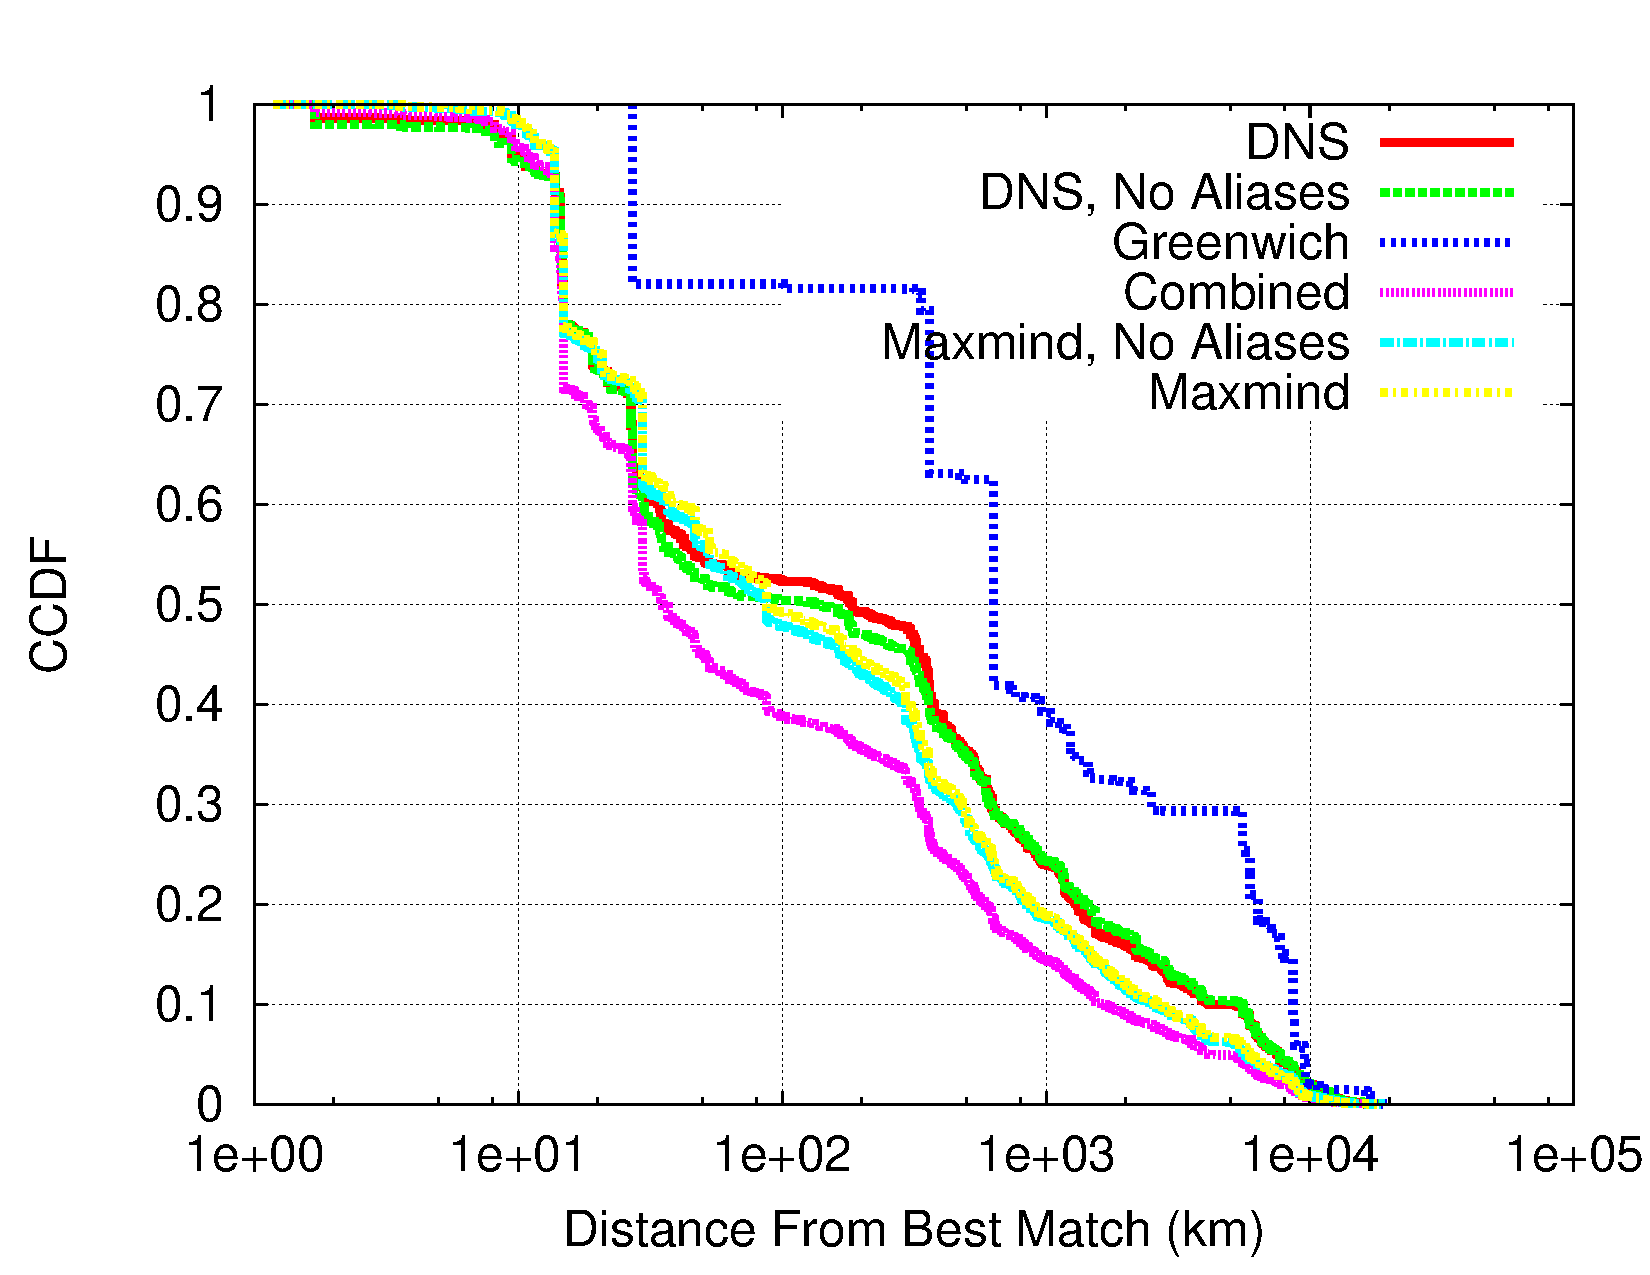
\includegraphics[width=3.25in]{graph_all_match_ccdf}
\caption[]{For ground truth peering locations, CCDF of distance to closest AS adjacency in our dataset using varying geolocation techniques. X-axis is in log scale.} 
%The $y$-axis is fraction of AS pairs with a path between them that traverses a service supporting AS. The $x$-axis is the fraction of ASes in the simulation topology supporting the service. }
%Using MIRO~\cite{miro} style multipath allows networks to provide access to services 
%even when their default path does not encounter a service-supporting AS.}
\end{figure}


